% Chapter 4

\chapter{Used Similarity Measures} % Main chapter title

\label{sim} % For referencing the chapter elsewhere, use \ref{Chapter1} 

\lhead{Chapter 4. \emph{Used Similarity Measures}} % This is for the header on each page - perhaps a shortened title

%----------------------------------------------------------------------------------------

This chapter is organized as follows Section ~\ref{lexicalsim} discusses the Lexical Similarity, semantic similarity is presented in section ~\ref{semanticSim}, which discuss corpus-based semantic similarity, and knowledge based similarity.

\section{Lexical Similarity}
\label {lexicalsim}
In linguistics, lexical similarity is a measure of the degree to which the word sets of two given languages  are similar. A lexical similarity of 1 (or 100\%) would mean a total overlap between vocabularies, whereas 0 means there are no common words.\\


\subsection{Document Represenatation}
\label {documentrep}
There are several ways to model a text document. For example, it can be represented as a bag of words, where words are assumed to appear independently and the order is immaterial. The bag of word model is widely used in information retrieval and text mining . Words are counted in the bag, which differs from the mathematical definition of set. Each word corresponds to a dimension in the resulting data space and each document then becomes a  vector consisting of non-negative values on each dimension. Here we use the frequency of each term as its weight, which means terms that appear more frequently are more important and descriptive for the document.
Let $D = \{d_1 , . . . , d_n \}$ be a set of documents and $T = \{t_1 , . . . ,t_m \}$ the set of distinct terms occurring in D. We discuss more precisely what we mean by "terms" below: for the moment just assume they are words. A document is then represented as a m-dimensional vector $t_d$.\\
Let tf (d, t) denote the frequency of term $t \,\epsilon\, T$ in document $d \, \epsilon\, D$. Then the vector representation of a document d is
\begin{equation}
\vec{t_{a}} = (tf(d,t_1),.....,tf(d,t_m))
\end{equation}
Although more frequent words are assumed to be more important as mentioned above, this is not usually the case in practice. For example, words like \RL{في , و ,ان} are probably the most frequent words that appear in Arabic text, but neither are descriptive nor important for the document’s subject. In fact, more complicated strategies such as the tfidf weighting scheme is normally used instead\citep{tfidf}.
\begin{figure}[htbp]
	\centering
		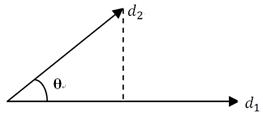
\includegraphics{./Figures/a.png}
		\rule{35em}{0.5pt}
	\caption[Angle Between Documents]{Angle Between Documents}
	\label{fig:Angle_Between_Documents}
\end{figure}
With documents presented as vectors, we measure the degree of similarity of two documents as the correlation between their corresponding vectors, which can be further quantified as the cosine of the angle between the two vectors.
Figure ~\ref{fig:Angle_Between_Documents} shows the angle in two-dimensional space but in practice the document space usually has tens and thousands of dimensions\citep{lexical}.

\subsubsection{Eculidean Distance}
\label {euclidean}
Euclidean distance is a standard metric for geometrical problems. It is the ordinary distance between two points and can be easily measured with a ruler in two- or three-dimensional space. Euclidean distance is widely used in clustering problems, including clustering text. It satisfies all the above four conditions and therefore is a true metric. It is also the default distance measure used with the K-means algorithm.\\
Measuring distance between text documents, given two documents $d_{a} and  d_{b}$ represented by their term vectors  $\overrightarrow{t_{a}} \,and\, \overrightarrow{t_{b}}$ respectively, the Euclidean distance of the two documents is defined as
where the term set is $T = {t1 , . . . , tm }$. As mentioned previously, we use the tf-idf value as term weights, that is
crucial for cluster analysis, especially for a particular type $w_{t,a} = tf idf (d_{a} , t)$.

\subsubsection{Cosine Similarity}
\label {cosine}
When documents are represented as term vectors, the similarity of two documents corresponds to the correlation between the vectors. This is quantified as the cosine of the angle between vectors, that is, the so-called cosine similarity. It is one of the most popular similarity measure applied to text documents, such as in numerous information retrieval applications and clustering too.
Given two documents $\overrightarrow{t_{a}} \,and\, \overrightarrow{t_{b}}$, their cosine similarity is

\begin{equation}
SIM_{c}(\vec{t_{a}},\vec{t_{b}}) =\frac{\vec{t_{a}}.\vec{t_{b}}}{|\vec{t_{a}}|\times|\vec{t_{b}}|}
\end{equation}

where $\overrightarrow{t_{a}} \,and\, \overrightarrow{t_{b}}$ are m-dimensional vectors over the term set $T = \{t1 , . . . , tm \}$. Each dimension represents a term with its weight in the document, which is non-negative. As a result, the cosine similarity is non-negative and bounded between [0,1].\\
An important property of the cosine similarity is its independence of document length. For example, combining two identical copies of a document $d$ to get a new pseudo document $d'$ , the cosine similarity between $d$ and $d'$ is 1, which means that these two documents are regarded to be identical. Meanwhile, given another document $l$, $d$ and $d'$ will have the same similarity value to l, that is, 
$SIM_{c}(\vec{t_{d}},\vec{t_{l}})= SIM_{c}(\vec{t_{d'}},\vec{t_{l}})$.\\ 
In other words, documents with the same composition but different totals will be treated identically. Strictly speaking, this does not satisfy the second condition of a metric,because after all the combination of two copies is a different object from the original document. However, in practice,when the term vectors are normalized to a unit length such as 1, and in this case the representation of $d$ and $d'$ is the same.

%----------------------------------------------------------------------------------------

\section{Semantic Similarity}
\label {semanticSim}
Measures of semantic similarity have been traditionally defined between words or concepts, and much less between text segments consisting of two or more words. The emphasis on word-to-word similarity metrics is probably due to the availability of resources that specifically encode relations between words or concepts (e.g. WordNet), and the various testbeds that allow for their evaluation (e.g. TOEFL or SAT analogy/synonymy tests). \\
Moreover, the derivation of a text-to-text measure of similarity starting with a word based semantic similarity metric may not be straightforward,and consequently most of the work in this area has considered mainly applications of the traditional vectorial model,occasionally extended to n-gram language models\citep{semantic}.\\

Given two input text segments, we want to automatically derive a score that indicates their similarity at semantic level,thus going beyond the simple lexical matching methods traditionally used for this task. Although we the fact that a comprehensive metric of text semantic similarity  should also take into account the structure of the text, we could model the semantic similarity of texts as a function of the semantic similarity of the component words. We do this by combining metrics of word-to-word similarity and word specificity into a formula that is a potentially good indicator of the semantic similarity of the two input texts.\\
   The following section provides details on some different corpus-based and knowledge-based measures of word semantic similarity. In addition to the similarity of words, we also take into account the specificity of words, so that we can give a higher weight to a semantic matching identified between two specific words (e.g. collie and sheepdog), and give less importance to the similarity measured between generic concepts 
(e.g. get and become).\\
Given a metric for word-to-word similarity and a measure of word specificity, we define the semantic similarity of two text segments $T1$ and $T2$ using a metric that combines the semantic similarities of each text segment in turn with respect to the other text segment. First, for each word $w$ in the segment $T1$ we try to identify the word in the segment $T2$ that has the highest semantic similarity $(maxSim(w, T2 ))$, according to one of the word-to-word similarity measures described in the following section~\ref{measuresSection}. Then, the same process is applied to determine the most similar word in $T1$ starting with words in $T2$ . The word similarities are then weighted with the corresponding word specificity, summed up, and normalized with the length of each text segment. Finally the resulting similarity scores are combined using a simple average. Note that only open-class words and cardinals can participate in this semantic matching process. As done in previous work on text similarity using vector-based models, all function words are discarded.
The similarity between the input text segments $T_1$ and $T_2$ is therefore determined using the following scoring function:
    
\begin{equation}
\label{simEq}
SIM({T_{1}},{T_{2}}) =\frac{1}{2}(\frac{\sum_{w\in \{T_1\}} (maxSim(w,T_2 * idf(w)))}{\sum_{w\in \{T_1\}} idf(w)} + \frac{\sum_{w\in \{T_2\}} (maxSim(w,T_1 * idf(w)))}{\sum_{w\in \{T_2\}} idf(w)})
\end{equation}

   This similarity score has a value between 0 and 1, with a score of 1 indicating identical text segments, and a score of 0 indicating no semantic overlap between the two segments.Note that the maximum similarity is sought only within classes of words with the same part-of-speech. The reason behind this decision is that most of the word-to-word knowledge-based measures cannot be applied across parts-of-speech, and consequently, for the purpose of consistency,we imposed the “same word-class” restriction to all the word-to-word similarity measures. This means that, for instance, the most similar word to the noun flower within the text “There are many green plants next to the house” will be sought among the nouns plant and house, and will ignore the words with a different part-of-speech (be, green, next). Moreover, for those parts-of-speech for which a word-to-word semantic similarity cannot be measured (e.g. some knowledge-based measures are not defined among adjectives or adverbs), we use instead a lexical match measure,which assigns a maxSim of 1 for identical occurrences of a word in the two text segments.
\subsection{Similarity Measures}
\label {SimilarityMeasures}
\label{measuresSection}
The Leacock \& Chodorow (Leacock \& Chodorow 1998) similarity is determined as:
\begin{equation}
SIM_{lch} = -log \frac{length}{2 \times D}
\end{equation}
where length is the length of the shortest path between two concepts using node-counting, and D is the maximum depth of the taxonomy.
The Lesk similarity of two concepts is defined as a function of the overlap between the corresponding definitions, as provided by a dictionary. It is based on an algorithm proposed by Lesk (1986) as a solution for word sense disambiguation.
The application of the Lesk similarity measure is not limited to semantic networks, and it can be used in conjunction with any dictionary that provides word definitions.
The Wu and Palmer (Wu \& Palmer 1994) similarity metric measures the depth of two given concepts in the WordNet taxonomy, and the depth of the least common subsumer (LCS), and combines these figures into a similarity score:
\begin{equation}
SIM_{wup} =\frac{2\times depth(LCS)}{depth(concept1) + depth(concept2)}
\end{equation}
The measure introduced by Resnik (Resnik 1995) returns the information content (IC) of the LCS of two concepts:
\begin{equation}
Sim_{res} = IC(LCS)
\end{equation}
where $IC$ is defined as:
$IC(c) = -log P(c)$ and $P(c)$ is the probability of encountering an instance of concept c in a large corpus.
The next measure we use in our experiments is the metric introduced by Lin (Lin 1998), which builds on Resnik’s measure of similarity, and adds a normalization factor consisting of the information content of the two input concepts:
\begin{equation}
SIM_{wup} =\frac{2\times IC(LCS)}{IC(concept1) + IC(concept2)}
\end{equation}
Finally, the last similarity metric considered is Jiang \& Conrath (Jiang \& Conrath 1997):
\begin{equation}
SIM_{jnc} =\frac{1}{IC(concept1) + IC(concept2) - 2\times IC(LCS)}
\end{equation}
Note that all the word similarity measures are normalized so that they fall within a 0–1 range. The normalization is done by dividing the similarity score provided by a given measure with the maximum possible score for that measure. 

\subsection{Corpus Based}
\label {corpus}
\subsubsection{LSA for Semantic Similarity}
LSA is a fully automatic mathematical/statistical technique for extracting and inferring relations of expected contextual usage of words in passages of discourse. It is not a traditional natural language processing or artificial intelligence program; it uses no humanly constructed dictionaries, knowledge bases, semantic networks, grammars, syntactic parsers, or morphologies, or the like, and takes as its input only raw text parsed into words defined as unique character strings and separated into meaningful passages or samples such as sentences or paragraphs.
Another way to think of this is that LSA represents the meaning of a word as a kind of average of the meaning of all the passages in which it appears, and the meaning of a passage as a kind of average of the meaning of all the words it contains. LSA's ability to simultaneously derive representations of these two interrelated kinds of meaning depends on an aspect of its mathematical machinery.\\

A rough analogy of how this can happen is as follows. Read the following sentence:\\
"John is Bob's father and Mary is Ann's mother." Now read this one: "Mary is Bob's mother."\\
Because of the relations between the words mother, father, son, daughter, brother and sister that you already knew, adding the second sentence probably tended to make you think that that Bob and Ann were brother and sister, Ann the daughter of John, John the father of Ann, and Bob the son of Mary, even though none of these relations is explicitly expressed (and none follow necessarily from the presumed formal rules of English kinship naming.) The relationships inferred by LSA are also not logically defined, nor are they assumed to be consciously rationalizable as these could be. Instead, they are relations only of similarityãor of context sensitive similarityãbut they nevertheless have mutual entailments of the same general nature, and also give rise to fuzzy indirect inferences that may be weak or strong and logically right or wrong\citep{lsa}.

\paragraph{How LSA works}
The first step is to represent the text as a matrix (the term-by-document matrix T)in which each row stands for a unique word and each column stands for a text passage or other context. Each cell contains the frequency with which the word of its row appears in the passage denoted by its column. Next, the cell entries are subjected to a preliminary transformation, whose details we will describe later, in which each cell frequency is weighted by a function that expresses both the word's importance in the particular passage and the degree to which the word type carries information in the domain of discourse in general.
Next, LSA applies singular value decomposition (SVD) to the matrix. This is a form of factor analysis, or more properly the mathematical generalization of which factor analysis is a special case. In SVD, a rectangular matrix is decomposed into the product of three other matrices. One component matrix (U) describes the original row entities as vectors of derived orthogonal factor values, another (V) describes the original column entities in the same way, and the third is a diagonal matrix (SIGMA) containing scaling values such that when the three components are matrix-multiplied, the original matrix (T) is reconstructed. 
There is a mathematical proof that any matrix can be so decomposed perfectly, using no more factors than the smallest dimension of the original matrix. When fewer than the necessary number of factors are used, the reconstructed matrix is a least-squares best fit. 

One can reduce the dimensionality of the solution simply by deleting coefficients in the diagonal matrix (SIGMA), ordinarily starting with the smallest. (In practice, for computational reasons, for very large corpora only a limited number of dimensions, currently a few thousands can be constructed). The SVD equations can be derived as follows\citep{lsa}:\\
\begin{equation}
\{X\} = \{W\}\{S\}\{P\}^T
\end{equation}

\paragraph{Stop-listing and stemming}
These are very rarely used. In keeping with the underlying theory and model, neither stemming nor stop-listing is appropriate or usually effective. As in natural language, the meaning of passages cannot be accurately reconstructed or understood without all of its words. However, when LSA is used to compare word strings shorter than normal text paragraphs, e.g. short sentences, zero weighting of function words is often pragmatically useful.
\paragraph{Similarity in the reduced space}
Since both passages (documents) and terms (words) are represented as vectors, it is straight forward to compute the similarity between passage-passage, term-term, and term-passage. In addition, terms and/or passages can be combined to create new vectors in the space. The process by which new vectors can be added to an existing LSA space is called folding-in. The cosine distance between vectors is used as the measure of their similarity for many applications because of its relation to the dot-product criterion and has been found effective in practice, although other metrics, such as Euclidean distance or City-Block (Manhattan) distance are sometimes used.

\paragraph{Shortfalls, objections, evidence and arguments}
potential limitations should be noted:
\begin{itemize}
\item [1.] It is likely, of course, that LSA's “bag of words” method, that ignores all syntactical, logical and nonlinguistic pragmatic entailments, sometimes misses meanings or gets it scrambled.
\item[2.] LSA became practical only when computational power and algorithm efficiency improved sufficiently to support SVD of thousands of words-by-thousands of contexts matrices; it is still impossible to perform SVD on the hundreds of thousands by tens of millions matrices that would be needed to truly represent the sum of an adult's language exposure.
\end{itemize}
Some commentators have also argued that LSA must be fundamentally wrong as theory because is not grounded in perception and intention. The strength of this objection is considerably reduced by the observation that language must veridically reflect these sources or it would be nearly useless, and by the human ability to generate, use and understand words as abstract and unrelated to perception as the word abstract itself, and by LSA’s varied successes.

Indeed, one should not think of LSA as a fixed mechanism or its representations as
fixed quantities, but rather, as evolving approximations.
%-------------------------------------------------------------------------------
\subsection{Knowledge Based}
\label {knowledge}
Evaluating semantic relatedness using network representations is a problem with a long history in artificial intelligence and psychology, dating back to the spreading activation approach of Quillian (1968) and Collins and Loftus (1975). Semantic similarity represents a special case of semantic relatedness: for example, cars and gasoline would seem to be more closely related than, say, cars and bicycles, but the latter pair are certainly more similar.\\
Rada et al.\citep{rada1989development} suggest that the assessment of similarity in semantic networks can in fact be thought of as involving just taxonomic (is-a) links, to the exclusion of other link types; that view will also be taken here, although admittedly links such as part-of can also be viewed as attributes that contribute to similarity.\\
    A natural, time-honored way to evaluate semantic similarity in a taxonomy is to measure the distance between the nodes corresponding to the items being compared - the shorter the path from one node to another, the more similar they are. Given multiple paths, one takes the length of the shortest one.\\
    A widely acknowledged problem with this approach, however, is that it relies on the notion that links in the taxonomy represent uniform distances. Unfortunately, uniform link distance is difficult to define, much less to control. In real taxonomies, there is wide variability in the "distance" covered by a single taxonomic link, particularly when certain sub-taxonomies (e.g., biological categories) are much denser than others. For example, in WordNet, broad-coverage semantic network for English, it is not at all difficult to find links that cover an intuitively narrow distance (rabbit ears is-a television antenna) or an intuitively wide one (phytoplankton is-a living thing). The same kinds of examples can be found in the Collins COBUILD Dictionary (Sinclair, ed., 1987), which identi es superordinate terms for many words (e.g.,safety valve is-a valve seems much narrower than knitting machine is-a machine)\citep{semantic_2}.\\

\subsubsection{AWN}
AWN is constructed according to the methods developed for EuroWordNet (EWN;Vossen 1998) and since applied to dozens of languages around the world. The EuroWordNet approach maximizes compatibility across wordnets and focuses on manual encoding of the most complicated and important concepts\citep{awn_0}. \\
Language-specific concepts and relations are encoded as needed or desired. This results in a so-called core wordnet for Arabic with the most important synsets, embedded in a solid semantic framework. From this core wordnet, it is possible to automatically extend the coverage with high precision. Specific concepts can be linked and translated with great accuracy because the base building blocks are manually defined and translated. \\
The approach follows a top-down procedure. Arabic Base Concepts are defined and extended via hyponymic relations to derive a core wordnet. The set of Common Base Concepts (CBCs) from the 12 languages in EWN and BalkaNet (Tufis 2004) are encoded as synsets; other language-specific concepts are added and translated manually to the closest synset(s) in Arabic. The same step is performed for all English synsets that currently have an equivalence relation in Suggested Upper Merged Ontology (SUMO).\\
The first layers of hyponyms are chosen on the basis of linguistic and applications based criteria; the final phase completes the target set of concepts/synsets, including specific domains and named entities. Each synset construction step is followed by a validation phase, where formal consistency is checked and the coverage is evaluated in terms of frequency of occurrence and domain distribution.\\

\paragraph{Structure and organization of AWN}
Because AWN is to be aligned not just to Princeton WordNet (PWN) (Fellbaum 1998) but to every wordnet aligned to PWN, the database design supports multiple languages, and the user interface will be explicitly multilingual rather than bilingual as was the one described in Black and Elkateb (2004)\citep{awn_1}.
The database structure comprises four principal entity types, item, word, form and link.
\begin{itemize}
\item [1.] Items are conceptual entities, including synsets, ontology classes and instances. Besides a unique identifier, an item has descriptive information such as a gloss. Items lexicalized in different languages are distinct.
\item [2.]A word entity is a word sense, where the citation form of the word is associated with an item via its identifier.
\item [3.]A form is a special form that is considered dictionary information (not merely an inflectional variant). The forms of Arabic words that go in this table are the root and/or the broken plural form, where applicable.
\item [4.]A link relates two items, and has a type such as "equivalence," "subsuming," etc. Links connect sense items to other sense items, e.g. a PWN synset to an AWN synset, a synset to a SUMO concept, etc.
\end{itemize}
This data model has been specified in XML as an interchange format, but is also implemented in a MySQL database hosted by one of the partners. The database will be the primary deliverable of the project, and will be distributed freely to the community.

\paragraph{Constructing AWN}
The basic criteria for selecting synsets to be covered in AWN are\citep{awn_2}: 
\begin{itemize}
\item Connectivity: AWN should be as densely connected as possible by hyperonymy / hyponymy chains, etc. Most of the synsets of AWN should correspond to English WN counterparts and the overall topology of both wordnets should be similar.
\item Relevance: Frequent and salient concepts have priority. Criteria will include the frequency of lexical items (both in Arabic and English) and the frequency of Arabic roots in their respective reference corpora.
\item Generality: Synsets on the highest levels of WN are preferred. These criteria suggest two ways for proceeding:
\item From English to Arabic: Given an English synset, all corresponding Arabic variants (if any) will be selected.
\item From Arabic to English: Given an Arabic word, all its senses have to be found, and for each of these senses the corresponding English synsets have to be selected.
\end{itemize}

Both steps have to be followed throughout the construction of AWN. All AWN synsets must be manually validated (and eventually locked, when all their variants have been found) but advantage should be taken as much as possible of the available resources for guiding the construction and validation process. Once a new Arabic verb is added to AWN, several possibilities for extension arise: extensions from verbal entries, including verbal derivatives, nominalizations, verbal nouns, etc. We also consider the most productive forms of deriving broken plurals. This can be done using a set of lexical and morphological rules. To take full advantage of these extensions short iterations will be performed. As stated in the introduction, the starting point of AWN is the manual construction of its Base Concept (BC) set from EWN and BalkaNet's CBCs. We concentrate on the most relevant terms for obtaining about 1,000 nominal and 500 verbal synsets. \\
The second step consists of the top-down vertical extension of BC, following Farreres 2005, Diab 2004). Some preprocessing is required for this and the next phase. We mention two tasks, preparation and extension. Preparation includes the processing of the available bilingual resources and the compilation of a set of lexical and morphological rules. From the set of available bilingual dictionaries we construct a homogeneous bilingual dictionary (HBIL) that contains for each entry information on the Arabic/English word pair, the Arabic root (added manually), POS, relative frequencies and sources supporting the pairing\citep{awn_2}.\\
The set of 17 heuristic methods used in the development of EWN will be applied to HBIL to derive candidate Arabic words/English synsets mappings. For each mapping the information attached includes the Arabic word and root, the English synset, POS, relative frequencies, mapping score, absolute depth in WN, number of gaps between the synset and the top of the WN hierarchy, and sources containing the pair.
Arabic words in bilingual resources must be normalized and lemmatized (Diab et al. 2004, Habash and Rambow 2005) but vowels and diacritics must be maintained. Arabic roots are not vowelized.
Following pre-processing, the set of scored Arabic word/English synset pairs becomes the input to the manual validation step. We proceed by chunks of related units (sets of related WN synsets, e.g. hyponymy chains and sets of related Arabic words, i.e., words having the same root) instead of individual units (synsets, senses, words).\\

\paragraph{Shortfalls of AWN:}
\begin{itemize}
\item High Coupling with UI\\
AWN suffers a very poor design that resulted in a high coupling between the Core Module and the Graphical User Interface (GUI) of the AWN, which made it very difficult to use the code module and the database without the GUI. However, we managed to decouple the GUI from the core modules of the AWN to allow its integration with other modules of semantic similarity. The decoupling process exerted a lot of time tracing and reverse engineering the code.
\item shortage of unique terms/word i.e there is so little number of words in database\\
       One reasonable limitation of AWN, assuming it is an initial version, is that it doesn’t contain a broad collection of Arabic words and terms. It contains only 17561 unique word, distributed among 7822 synsets.This leads to a lot of missing words that have no record in AWN’s database. e.g. \RL{جنوب افريقيا, أحمد, محمد}
\item Running time is major problem\\
Since AWN depends on the Tree Concept (a hierarchical organization of the synsets), it has an arabic tree with nodes that represent synsets, each synset contains set of words. So every time the AWN is queried by a term, in order to retrieve its synset, the whole tree is first searched for this term. If the term was not found in the tree, we seek it from database. If the term is found in the database, then the retrieved results from the database would include the path of the term in the hierarchical tree. The final step, that is to expand the retrieved path into the tree, exhausts a substantial amount of time. The time consumption is due to the way the path expansion work. \\
The path expansion starts at the tree root node and traverses the tree through the path retrieved from the database. If a node on the path was not found in the current tree, the node is added to the tree and all its children are fetched from the database and added to the tree. The last step consumes a lot of time because it expands all the node’s children, although only one child is needed. This caused the tree expansion for some words to consume up to 15 minutes.\\
Another issue that consumes a lot of time is the path retrieval from the database. When a term needs to be fetched from the database, first its synset needs to be find. After the synset is found, the path of the synset in the hierarchical tree also needs to be found. The path is assembled starting from the term’s synset traversing its parent up until the root is reached (you can think of the process traversing up the tree using Forwarding Pointers). \\
\item Bugs in the code\\
\begin{itemize}
\item There was missing logic in the code probably because these methods were never called by the GUI.
\item There was some missing constants in the core of AWN, it can't recognize some patterns of words
\end{itemize}
\end{itemize}
  
\paragraph{What we have done}
\begin{itemize}
\item We managed to decouple the Code module from the GUI to be able to use each one separately.
\item We fixed some bugs in the code.
\begin{itemize}
\item Missing logic in the code
\item Missing constants
\end{itemize}
\item we modified the expansion algorithm and managed to reduce expansion time to 20\% of the original running time.
\end{itemize}

\textit{How we Use it?}\\
\textit{Wu and Palmer}\\
    If words can be defined with concepts in a hierarchical structure, it is possible to measure the meaning similarity between words with an information measure based on WordNet (Resnik,1993), or structure level information based on a thesaurus (Kurohashi and Nagao, 1992). How-
ever, verb meanings are difficult to organize in a hierarchical structure.\\
In each conceptual domain, lexicalized concepts can be organized in a hierarchical structure. Within one conceptual domain, the similarity of two concepts is defined by how closely they are related in the hierarchy, i.e., their structural relations.\\
The Wu and Palmer \citep{wu} similarity metric measures the depth of two given concepts in the WordNet taxonomy, and the depth of the least common subsumer (LCS), and combines these figures into a similarity score:
\begin{equation}
\label{wu_palmer}
SIM({T_{1}},{T_{2}}) =\frac{2 * depth(LCS)}{depth(concept_1)+ depth(concept_2)} 
\end{equation}

so we utilized the Wu\&Palmer Technique and AWN to measure the semantic similarity according to the following stpes:
\begin{itemize}
\item [1.] Search for both terms in the Arabic Tree in the AWN if found get there’s  depth and their least common ancestor.
\item [2.] if not found search database to get their synsets and expand them in the tree. This is the most expensive operation in the whole procedure due to the database request also due to the expansion operation.
\item [3.] then get the depths of both synsets and their least common ancestor 
\item [4.] Finally use Wu and Palmer to get the similarity using the Wu and Palmer equation ~\ref{wu_palmer}
\item [5.] Apply the semantic similarity equation ~\ref{simEq}
\end{itemize}

\subsubsection{Wikipedia}
Using the traditional approach of a controlled, designed ontology has many disadvantages beginning with the often difficult task of designing and implementing the ontology. Once that it done, it must be maintained and modified, an important process in domains where the underlying concepts are evolving rapidly. ACM’s CCS, for example, undergoes periodic reorganization and redesign and yet as a classification of computer science concepts, it always seems to be out of date or even quaint. As a final problem, consider the process a person must follow in assigning ontology terms to a document. She has to be familiar with all of the possible choices or have some way to browse or search through them. She has to understand what each of the terms means, either the original meaning intended by the ontology designer or the possibly different current meaning as used by her community. Finally, she has to select the best set of terms from among the many relevant choices the ontology may present to her. The use of an implicit ontology emerging from the tagging choices of a community of individuals solves some of these problems, but also has significant disadvantages\citep{wiki_1}.\\
Some of these are inherent and others are being addressed in the research community and may ultimately admit good solutions. These problems are worth addressing because the result will be an ontology that 
\begin{itemize} \item [(1)] represents a consensus view of a community of users and \item [(2)]  is constructed and maintained by the community without cost to any organization. 
\end{itemize}
It remains unclear how the terms in such an ontology should be organized structurally, understood informally by end users, or mapped to a more formal ontology such as Cyc (Lenat 1995) or popular Semantic Web ontologies like FOAF (Ding et al. 2005). 
We are developing a system that is a blend of the two approaches based on the idea of using Wikipedia as an ontology. Specifically, each non-administrative Wikipedia page is used as a term in an ontology. These include Wikipedia articles describing individuals (Alan Turing), concepts (Emissions trading), locations (Barbados), events (collapse of the World trade Center), and categories (microbiology). 
Using Wikipedia as an ontology has many advantages: it is broad and fairly comprehensive, of generally high quality, constructed and maintained by tens of thousands of users, evolves and adapts rapidly as events and knowledge change, and free and “open sourced”. Moreover, the meaning of any term in the ontology is easy for a person to understand from the content on the Web page. Finally, the Wikipedia pages are already linked to many existing formal ontologies through efforts like DBpedia (Auer et al. 2007) and Semantic MediaWiki (Krotzsch et al. 2006) and in commercial systems like Freebase and Powerset.\\
The underlying concept of an article cannot be assessed by merely considering the words that appear in that article, in addition to that, finding out if two articles are conceptually related is an even more challenging problem and requires a lot of background domain knowledge, common sense as well as information about the context. Humans have the inborn ability to relate concepts semantically however it is still a very difficult problem for computers, which can be made easier by augmenting background domain knowledge for such tasks, which would certainly improve the accuracy and quality of prediction. Wikipedia proves to be an invaluable source for such background domain knowledge.\\

Wikipedia is a freely available online encyclopedia developed by a community of users. Wikipedia is growing exponentially and new content is being added to it daily by users around the globe. This encyclopedia comprises of millions of articles. The corpus is composed of several collections in different languages such as: English, French, German, Dutch, Chinese, Spanish, Arabic and Japanese. \\
Each collection is a set of XML documents built using Wikipedia. Documents of the Wikipedia XML collections are organized in a hierarchy of categories defined by the authors of the articles. The Wikipedia category and article network has been studied in detail with respect to different graph properties. The Wikipedia category system is a taxonomy for arranging articles into categories and subcategories.\\
However, this taxonomy is not a strict hierarchy or tree of categories, but allows multiple categorizations of topics simultaneously, i.e., some categories might have more than one super-category. It is shown that Wikipedia’s category system is a thesaurus that is collaboratively developed and used for indexing Wikipedia articles (Voss 2006). The articles within Wikipedia are inter-linked. However, these links do not impose any subcategory or super-category relationships. It has been observed that the Wikipedia article links graph generally resembles the World Wide Web graph.\\

\paragraph{Lucene}
We used lucene to buuild an inverted index on whole Wikipedia Articles, so we could be able to search for any term within the wikipedia aricles efficiently, aslo to get the search results ranked according to the search query.\\
Here is some Sample code for how we used Lucene the following one is sample indexing code, where Document object represents Wikipedia Articles to be indexed, Also ArabicAnalyzer is the Analyzer we used as it uses the light stemmer as we do in the datasets we used in our experiments.\\

\lstset{ %
  language=Java,                % the language of the code
  basicstyle=\footnotesize,           % the size of the fonts that are used for the code
  numbers=left,                   % where to put the line-numbers
  numberstyle=\tiny\color{gray},  % the style that is used for the line-numbers
  stepnumber=2,                   % the step between two line-numbers. If it's 1, each line 
                                  % will be numbered
  numbersep=5pt,                  % how far the line-numbers are from the code
  backgroundcolor=\color{white},      % choose the background color. You must add \usepackage{color}
  showspaces=false,               % show spaces adding particular underscores
  showstringspaces=false,         % underline spaces within strings
  showtabs=false,                 % show tabs within strings adding particular underscores
  frame=single,                   % adds a frame around the code
  rulecolor=\color{black},        % if not set, the frame-color may be changed on line-breaks within not-black text (e.g. commens (green here))
  tabsize=2,                      % sets default tabsize to 2 spaces
  captionpos=b,                   % sets the caption-position to bottom
  breaklines=true,                % sets automatic line breaking
  breakatwhitespace=false,        % sets if automatic breaks should only happen at whitespace
  title=\lstname,                   % show the filename of files included with \lstinputlisting;
                                  % also try caption instead of title
  keywordstyle=\color{blue},          % keyword style
  commentstyle=\color{dkgreen},       % comment style
  stringstyle=\color{mauve},         % string literal style
  escapeinside={\%*}{*)},            % if you want to add a comment within your code
  morekeywords={*,...}               % if you want to add more keywords to the set
}
\begin{lstlisting}
MaxFieldLength mlf = MaxFieldLength.UNLIMITED;
ArabicAnalyzer analyzer = new ArabicAnalyzer(Version.LUCENE_35);
IndexWriter writer = new IndexWriter(directory, analyzer, true, mlf);
Document doc;
doc = new Document();
doc.add(new Field("url", br.readLine(),	Field.Store.YES,Field.Index.NOT_ANALYZED));
doc.add(new Field("title", line,Field.Store.YES,Field.Index.ANALYZED, Field.TermVector.YES));
doc.add(new Field("contents", br.readLine(),Field.Store.YES,Field.Index.ANALYZED, Field.TermVector.YES));
writer.addDocument(doc);
writer.close();
\end{lstlisting}

While this code Snippet represents sample for searching the inverted index for a certain term that occured in the Contents of any document in the inverted index.\\

\begin{lstlisting}
IndexReader reader = IndexReader.open(new SimpleFSDirectory(new File("Index")));
TermDocs documents;
Term term = new Term("contents", doc[i]);
documents = reader.termDocs(term);
reader.docFreq(term);
documents.read(docs, freqs);
\end{lstlisting}

We downloaded the Wikipedia XML snapshot of 21 June 2011 and extracted around 450,000 Wikipedia articles. The text of each article was indexed using the Lucene text search engine library \citep{lucene} under the standard configuration. We also downloaded the Wikipedia database tables in order to create the category links graph and the article links graph.\\
\begin{figure}[htbp]
	\centering
		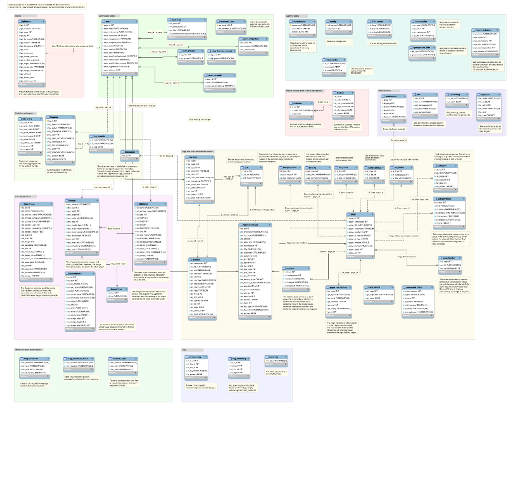
\includegraphics{./Figures/wiki_DB.png}
		\rule{35em}{0.05pt}
	\caption[Wikipedia Database Schema]{Wikipedia Database Schema}
	\label{fig:Wikipedia Database}
\end{figure}
\textit{How we Use it}\\
We have managed to implement two techniques based on the wikipedia structure as an Ontology, First technique we treated the Wikipedia Articles as Concepts\citep{wiki_1},then Every Document is represented with a vector containg around 450,000 concepts.
For each term $w_i$ in document $d_1$ we search the wikipedia articles using the inverted index built by Lucene ~\ref{luceneTool} and get vector of Articles or Concepts $V = \{c_1,c_2,...,c_n\}$, for every result lucene returns $c_i$, this term $w_i$ votes for every Article (concept  vector $V$ in the document vector where it was found by the $TF-IDF$ value in this Article.
finally we have a vetocr $d =\{\sum_{i=0}^{N} tfidf(w_1,c_i),\sum_{i=0}^{N} tfidf(w_2,c_i),...\sum_{i=0}^{N} tfidf(w_n,c_i)\} $ that represents each document we have then we apply cosine similarity to these vectors to calculate similarities ~\ref{cosine}.\\
\begin{figure}[htbp]
	\centering
		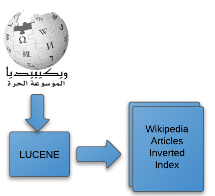
\includegraphics{./Figures/wiki_1.png}
		\rule{35em}{0.05pt}
	\caption[Wikipedia Indexing]{Wikipedia Indexing}
	\label{fig:Indexing}
\end{figure}

\begin{figure}[htbp]
	\centering
		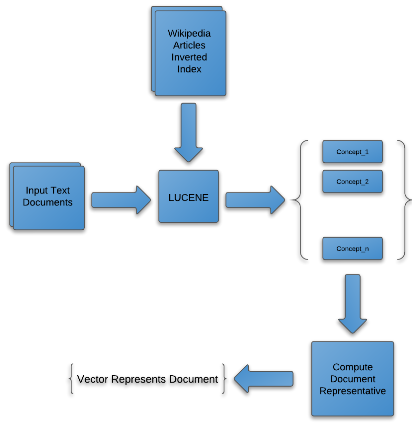
\includegraphics{./Figures/wiki_3.png}
		\rule{35em}{0.05pt}
	\caption[Wikipedia Method one]{Wikipedia Method one}
	\label{fig:Method one}
\end{figure}

\paragraph{Drawbacks}	
\begin{itemize}
\item High Dimensionality may lead to inaccurate or even incorrect results due to the sparse vectors comparison.
\item Long Running time, however it's not too long like the AWN-based Technique. 
\end{itemize}
To Overcome these problems we faced we tried two improvments on this technique, first we tried to compute the global uniopn vector for each dataset we used in the experiments to truncate those concepts that never appeared in our dataset to avoid any misleading values.With this modification only we managed to reduce the 450,000 concepts to around 8600 concepts.\\
second we applied the PCA ~\ref{pca} to reduce the high dimensionality, however this technique introduced another problem that PCA matrix result from the decomposition may contains negative values leading to negative similarities values.
To solve this new problem we tried the Automated contrast Adjustment Technique \citep{acadjstment} a used the folowing equation to map the range [-1,1] of cosine probable output and the desired range [0,1].
\begin{equation}
f(a) =a_{min}+ (a- a_{low})\times \frac{a_{max}-a_{min}}{a_{high} - a_{low}}
\end{equation}

Concerning Second Approach using the Wikipedia,We utilized the wikipedia Database ~\ref{wiki_DB} and used the categories each articles belongs to to be our concepts instead of the Article it'self. Our scoring scheme was simply count the number of times that each Wikipedia category was associated with one of the N results returned by lucene ~\ref{lucene} inverted index \citep{wiki_2}.
\begin{figure}[htbp]
	\centering
		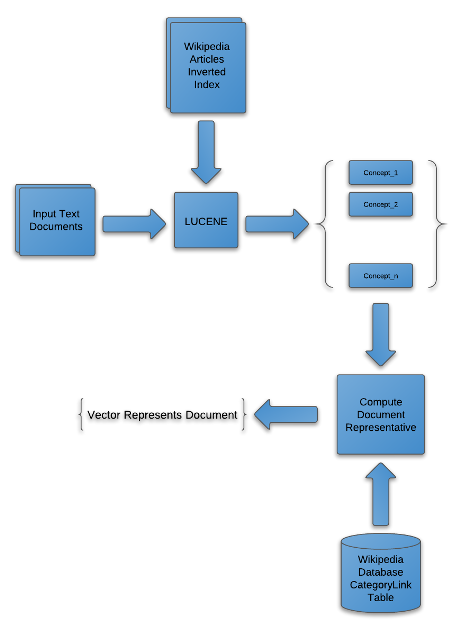
\includegraphics{./Figures/wiki_2.png}
		\rule{35em}{0.05pt}
	\caption[Wikipedia Method Two]{Wikipedia Method Two}
	\label{fig:Method Two}
\end{figure}
\subsection{Term Weigthing using Specificity}
The following section provides more insight into term Specificity, which is the idea that some words carry more semantic content than others which is also referred to as Semantic Informativeness. Computational estimation of this quantity, term specificity, is important for various applications such as information retrieval. Here in addition to the similarity of words, we also take into account the specificity of words, so that we can give a higher weight to a semantic matching identified between two specific words (e.g. collie and sheepdog), and give less importance to the similarity measured between generic concepts (e.g. get and become).\\
 While the specificity of words is already measured to some extent by their depth in the semantic hierarchy, we are reinforcing this factor with a corpus-based measure of word specificity, based on distributional information learned from large corpora.
We use two methods of computing term specificity. The first method based on modeling the rate of learning of word meaning in Latent Semantic Analysis (LSA), LSA-Specificity. The second method is TF/IDF-Specificity\citep{spec}.

\subsubsection{Latent Semantic Analysis:}
In the following section we explain using Latent Semantic Analysis for approximating term Informativeness. Latent Semantic Analysis (LSA) is a language model that represents semantic word meaning as vectors in high-dimensional space. Word vectors are positioned in such a way that semantically-related words vectors point in similar directions or have a smaller angle / higher cosine between them. The representation is derived in an unsupervised manner, by observing occurrence patterns of words in a large corpus of natural language documents. Singular Value Decomposition (SVD) on the matrix of word/document occurrence counts is used to derive the optimal set of dimensions of the space in which all of the words can be represented as vectors. The number of dimensions is then artificially reduced to a smaller number (typically around 300) of most important dimensions, which has the effect of smoothing out incidental relationships and preserving significant ones between words. The resulting geometric space allows for straightforward representation of meaning of words and/or documents; the latter are simply a weighted geometric composition of constituent word vectors. Similarity in meaning between a pair of words or documents can be obtained by computing the cosine between their corresponding vectors. For details of LSA, please see (Landauer et al., 2007), and others.\\
LSA applications almost always focus on computing the semantic similarity between words (terms). However, another property of LSA, that has a significant effect, is the term vector length. The vector length plays a very important role in many LSA calculations, in particular – in giving relative weights to the word vectors that constitute a particular text passage. As (Kintsch, 2001) wrote, “Intuitively, the vector length tells us how much information LSA has about this vector. [...] Words that LSA knows a lot about (because they appear frequently in the training corpus [...]) have greater vector lengths than words LSA does not know well. Function words that are used frequently in many different contexts have low vector lengths -- LSA knows nothing about them and cannot tell them apart since they appear in all contexts”.
The metric of term Informativeness, or specificity, which we call LSAspec, is simply the ratio of LSA word vector length to the number of documents in the LSA training corpus that contain a particular word;
\begin{equation}
LSAspec(w)=\frac{\| \overrightarrow{w}\|}{df_w}
\end{equation}
The value can be interpreted as the rate of vector length growth. We argue that more specific, or informative, words have the greatest rate of vector length growth; LSA learns about their meaning faster, with relatively fewer exposures. To illustrate this concept, let's look at a few examples that were obtained by controlling the number of occurrences of a particular word in the LSA training corpus. \\
@Mohsen: Should provide a graph for the relation of Vector lengths for some words vs. the number of documents containing those words.\\

\subsubsection{Inverse Document Frequency:}
The specificity of a word is determined using the inverse document frequency (IDF) introduced by (Sparck-Jones, 1972), defined as the total number of documents in the corpus divided by the total number of documents including that word. The IDF measure was selected based on previous work that theoretically proved the effectiveness of this weighting approach (Papineni, 2001). Sparck Jones (1973) defines IDF as the probability of occurrence of documents containing a particular word.\\
IDF equation and definition of its terms\\
Where D is the total number of documents in the corpus. The assumption behind it is that low frequency words tend to be rich in content, and vice versa.
The term count in the given document is simply the number of times a given term appears in that document. This count is usually normalized to prevent a bias towards longer documents (which may have a higher term count regardless of the actual importance of that term in the document) to give a measure of the importance of the term t within the particular document d. One well-studied technique is to normalize the TF weights of all terms occurring in a document by the maximum TF in that document\citep{tfidf_1}.\\
%----------------------------------------------------------------------------------------
\subsection{Disambiguation}                                            
Word Sense Disambiguation (WSD) is traditionally considered an AI-hard problem.A breakthrough in this field would have a significant impact on many relevant web-based applications, such as information retrieval and information extraction. next Section ~\ref{jigsawSec} describes JIGSAW, a knowledge-based  WSD algorithm that attemps to disambiguate all words in a text by exploiting WordNet senses. The main assumption is that a specific strategy for each Part-Of-Speech (POS)  is better than a single strategy.\\
Participants disambiguate text by assigning WordNet synsets, then the  system has to do the expansion to other languages, index the expanded documents and run the retrieval for all the languages in batch. The retrieval results are taken as a measure for the effectiveness of the disambiguation.

\subsubsection{JIGSAW Algorithm\citep{disambiguation}}
\label{jigsawSec}
The goal of a WSD algorithm consists in assigninga word wi occurring in a document d with its appropriate meaning or sense s, by exploiting the context $C$ in where wi is found. The context C for wi is defined as a set of words that precede and follow $w_i$ .The sense s is selected from a predefined set of possibilities, usually known as sense inventory. In the proposed algorithm, the sense inventory is obtained from WordNet, according to SemEval-2007 task 1 instructions. \\
JIGSAW is a WSD algorithm based on the idea of combining three different strategies to with sense sij . The intuition behind this algorithm disambiguate nouns, verbs, adjectives and adverbs.The main motivation behind our approach is that the effectiveness of a WSD algorithm is strongly influenced by the POS tag of the target word. An adaptation of Lesk dictionary-based WSD algorithm has been used to disambiguate adjectives and adverbs (Banerjee and Pedersen, 2002), an adaptation of the Resnik algorithm has been used to disambiguate nouns (Resnik, 1995), while the algorithm we developed for disambiguating verbs exploits the nouns in the context of the verb as well as the nouns both in the glosses and in the phrases that WordNet utilizes to describe the usage of a verb. \\
JIGSAW takes as input a document $d = {w_1 , w_2 , . . . , w_h }$ and returns a list of WordNet synsets $X = {s_1 , s_2 , . . . ,s_k }$ in which each element si is obtained by disambiguating the target word wi based on the information obtained from WordNet about a few immediately surrounding words. We define the context C of the target word to be a window of n words to the left and another n words to the right, for a total of $2n$ surrounding words. The algorithm is based on three different procedures for nouns, verbs, adverbs and adjectives, called JIGSAWnouns , JIGSAWverbs , JIGSAWothers , respectively. More details for each one of the above mentioned procedures follow.


\subsection{Principal component analysis}\label{pca}
Principal component analysis (PCA) is a multivariate technique that analyzes a data table in which observations are described by several inter-correlated quantitative dependent variables. Its goal is to extract the important information from the table, to represent it as a set of new orthogonal variables called principal components, and to display the pattern of similarity of the observations and of the variables as points in maps. \\
The quality of the PCA model can be evaluated using cross-validation techniques such as the bootstrap and the jackknife. PCA can be generalized as correspondence analysis (CA) in order to handle qualitative variables and as multiple factor analysis (MFA) in order to handle heterogeneous sets of variables. Mathematically, PCA depends upon the eigen-decomposition of positive semi-definite matrices and upon the singular value decomposition (SVD) of rectangular matrices.\cite{pca}
